\documentclass[fleqn]{jbook}
\usepackage{physpub}
\usepackage{txfonts}

\begin{document}
\begin{question}{問題8}{山地洋平}
図1は、ある球状タンパク質の熱転移(熱によるアンフォールディング転移)を、示差走査型熱量計と230nmにおける円二色性を用いて測定した結果を示す。測定は1気圧の一定圧力下にて行った。Aは、タンパク質水曜鋭気の熱量計データ、Bはタンパク質を溶かした緩衝溶液の熱量計データ、Cは円二色性の温度依存性を示す。図1のデータより、温度$T$におけるアンフォールディング転移の熱力学量(標準Gibbs自由エネルギー変化$\Delta G(T)$エンタルピー変化$\Delta H(T)$エントロピー変化$\Delta S(T)$など)を求めることができる。図2は、このようにして得られた熱力学量をもとにして、$\Delta G$の温度依存性を描いた理論曲線である。以下の問に答えよ。ただし、このタンパク質の熱転移は二状態転移で近似できるものとする。
\begin{figure}[htbp]
\begin{center}
%\includegraphics[width=.7\linewidth]{2002phy8q1.eps}
\includegraphics[width=.7\linewidth]{2002physQ8_1.eps}
\caption{ある球状タンパク質の熱転移。A:示差走査型熱量計による測定結果。B:示差走査型熱量計のベースライン(Aと同じ測定を溶媒緩衝液に対して行った)。C:円二色性の測定結果(点は測定点、実線は転移曲線を示す)。}
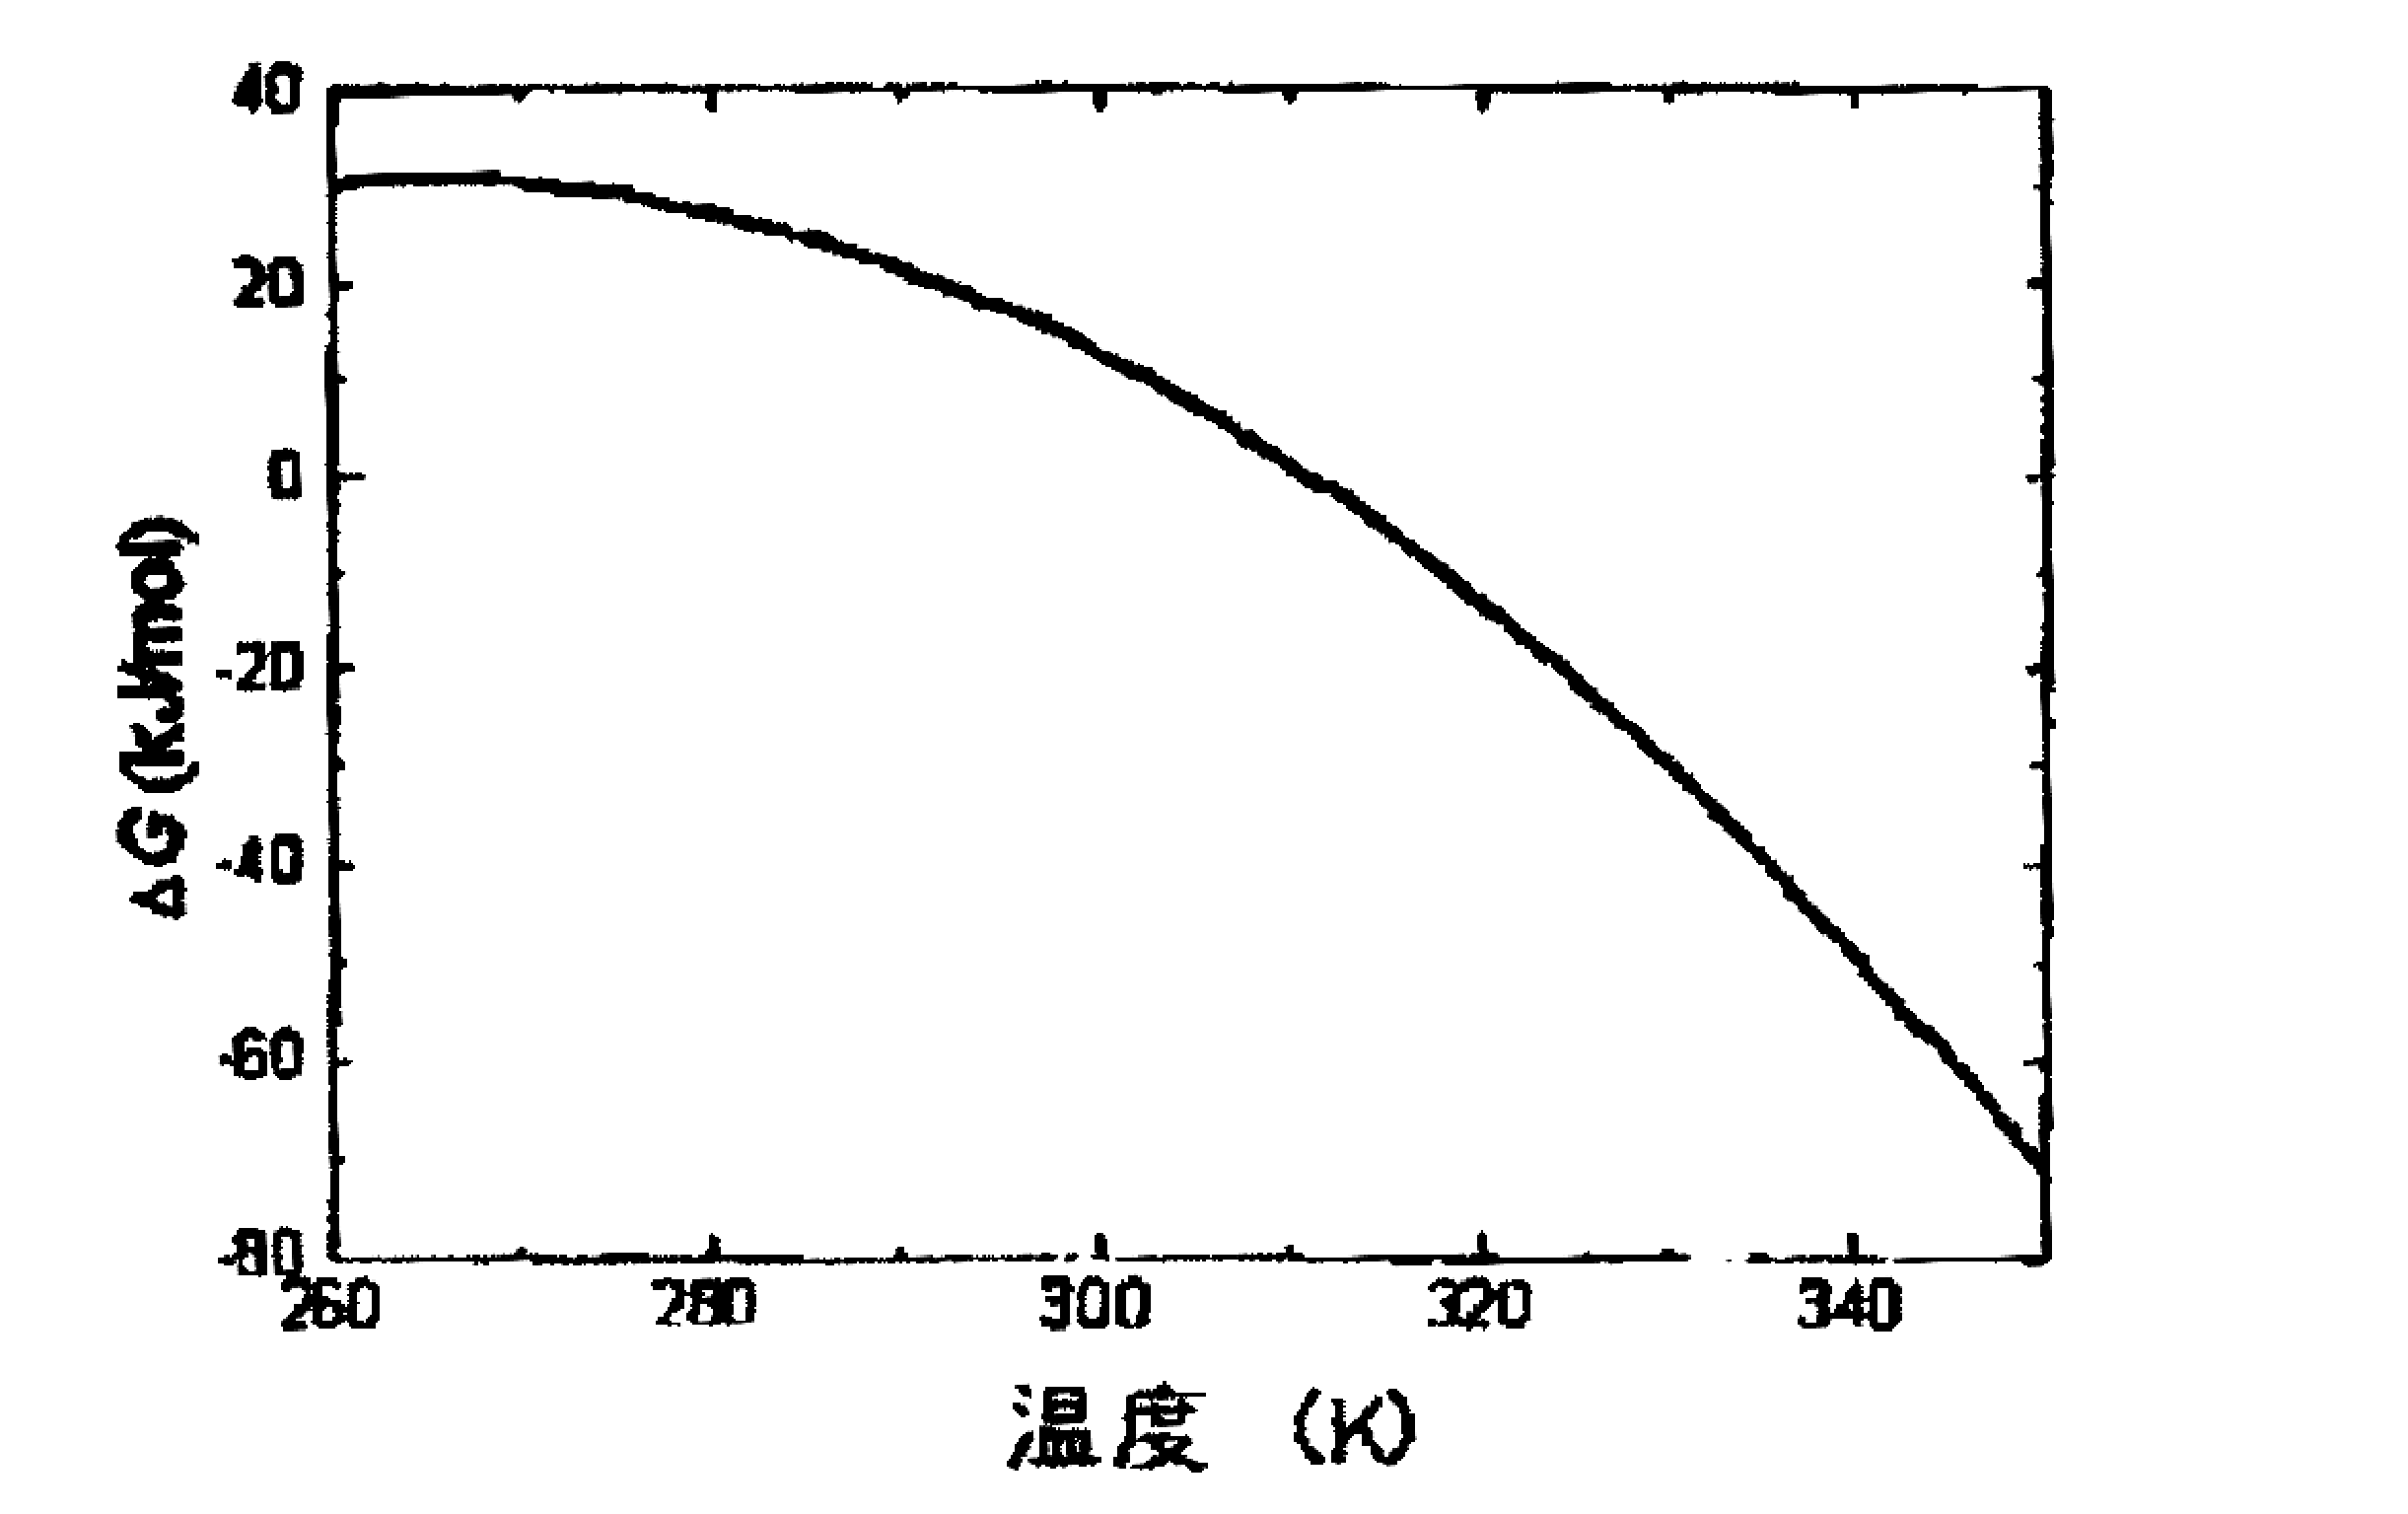
\includegraphics[width=.7\linewidth]{2002phy8q2.eps}
\caption{$\Delta G$の温度依存。}
\end{center}
\end{figure}
\newpage
\begin{enumerate}
\item 二次相転移が成立するので、図1中のCの転移曲線より転移前後の円二色性の温度依存を直線的に外挿し、転移領域での転移の割合$f_{\mathrm{app}}$を
$f_{\mathrm{app}}=b/(a+b)$として求めることができる(下図参照)。このとき、転移領域における転移の平衡定数$K$と標準自由エネルギー変化$\Delta  G$はどのように与えられるかを示せ。
\begin{figure}[htbp]
\begin{center}
%\includegraphics[width=.4\linewidth]{2002phy8q3.eps}
\includegraphics[width=.4\linewidth]{2002physQ8_3.eps}
\end{center}
\end{figure}
\item 平衡定数$K$と熱転移のvant' Hoffエンタルピー変化$\Delta H_{\mathrm{vH}}$に関する以下の関係式
\begin{eqnarray}
\Delta H_{\mathrm{vH}}=RT^2\frac{\partial \ln K}{\partial T}
\end{eqnarray}
を導け。ただし、ここで$R$は気体定数を表す。必要であれば、自由エネルギーとエンタルピーおよびエントロピーに関する関係式$\Delta G=\Delta H-T\Delta S$を用いてよい。
\item 熱量計により直接観測したエンタルピー変化$\Delta H_{\mathrm{cal}}$を図1中のAとBより求めることができる。その方法について、必要であれば図を描いて、説明せよ。
\item $\Delta H_{\mathrm{vH}}$と$\Delta H_{\mathrm{cal}}$の間にはどのような関係が成立するか。また、熱転移が二状態間転移では近似できず、中間状態を伴う場合、これらの間の関係はどうなるか。
\item 熱転移点の温度$T_m$、熱転移に伴う定圧熱容量変化$\Delta C_p$とし、$C_p$は温度に依らず一定と見なすことができる。このとき、任意の温度$T$における、自由エネルギー変化$\Delta G(T)$は以下の関係式で表されることを示せ。
\begin{eqnarray}
\Delta G(T) = \Delta H(T_m) + \Delta C_p\cdot(T-T_m) - T\left( \Delta S(T_m) + \Delta C_p \ln\frac{T}{T_m} \right)
\end{eqnarray}
\item 図1中のCのデータでは、230nmの円二色性の強度が熱転移に伴って減少している。円二色性とタンパク質の立体構造との関係について述べ、熱転移に伴う円二色性の変化が立体構造のどのような変化によりもたらされたかを説明せよ。
\item タンパク質の熱転移は、一般に、大きな$\Delta C_p$を伴うため、$\Delta G$の温度依存には図2のような曲率が生じ、タンパク質は$T_m$における熱転移とともに、低温側の$T_c$においても冷却転移を示す($T_c$が水の氷点より低くなり、現実には観測できないことが多い)。タンパク質の熱転移と冷却転移の起こる分子的なメカニズムについて、それぞれ、知れることを述べよ。
\end{enumerate}
\end{question}
\begin{answer}{問題8}{山地洋平}
\begin{enumerate}
\item
物質$k$の一分子当たりの標準自由エネルギーを$\mu^{\ 0}_{k} (T)$,\ 一分子当たりの自由エネルギーを$\mu _{k} (T,p)$とおくと,\
活量$a_{k}$は以下の式で定義される:
\begin{eqnarray}
\mu_{k} (T,p) = \mu^{\ 0}_{k} (T) + k_{B}T\ln a_{k}. \ilabel{eq.1}
\end{eqnarray}
また,\ 物質$k$と物質$k'$の間での\underline{二状態転移における}平衡定数$K(T)$は次式で定義される:
\begin{eqnarray}
K(T) = \frac{a_{k'}}{a_{k}}. \ilabel{eq.2}
\end{eqnarray}
\quad 反応系を理想溶液で近似すると,\ 活量はモル分率によって近似される.\ すなわち,\ 所与の転移の割合$f_{app}$を用いて,\
平衡定数は次のように計算される:
\begin{eqnarray}
K(T) = \frac{f_{app}}{1-f_{app}}.
\end{eqnarray}
一方で式(\iref{eq.1}),\ (\iref{eq.2})より,\
\[
K(T) = \exp
\left( \frac{ \mu_{k'} (T,p) - \mu^{\ 0}_{k'} (T) - \left(\mu_{k} (T,p) - \mu^{\ 0}_{k} (T) \right)  }{ k_{B} T }  \right),
\]
となるが,\ 各温度において熱平衡状態に達していたのであれば,\ $\mu_{k} (T,p) = \mu_{k'} (T,p)$が成り立つ.\ これより上の式は
以下のように変形できる:
\begin{eqnarray}
K(T) = \exp
\left(  -\frac{ \mu^{\ 0}_{k'} (T) - \mu^{\ 0}_{k} (T)  }{ k_{B} T }  \right).
\end{eqnarray}
以上から標準自由エネルギー$\Delta G$は分子数$N$と転移の割合$f_{app}$によって,\
\begin{eqnarray}
\Delta G &=& N \left(\mu^{\ 0}_{k'} (T) - \mu^{\ 0}_{k} (T) \right), \ilabel{eq.5} \\
&=&-N k_{B} T \ln K(T) ,\nonumber\\
&=&\displaystyle  RT \ln\frac{1-f_{app}}{f_{app}},\nonumber
\end{eqnarray}
と計算される.\ ただし,\ 得られた $\Delta G$は二状態転移を仮定しているため,\ model\ dependentである.
\item
Gibbsの自由エネルギーは,\ $G=H-TS$によって表されるので,\
\[
S=-\frac{\partial G}{\partial T},
\]
が成り立つ.\ 故に,\ 偏微分の線形性から,\
\begin{eqnarray}
\Delta S = -\frac{\partial \Delta G}{\partial T}.
\end{eqnarray}
$\Delta G= \Delta H- T \Delta S$を,\ 上の式と式(\iref{eq.5})の二行目を用いて変形すると,\
\begin{eqnarray}
\Delta H &=& - R T \ln K +  T\frac{\partial}{\partial T}R T \ln K, \\
&=&R T^{2}\frac{\partial \ln K}{\partial T},\nonumber
\end{eqnarray}
が得られる.\ これは二状態転移を前提としたvan't\ Hoffのエンタルピー変化に他ならない.
\item
溶液のDSCの読みから溶質のDSCの読みを引いた上に,
\ $C_{p}$の変化によって生じるback\ groundを引く.\
残されたピークの面積が$\Delta H_{cal}$となる.\par
$\Delta H_{cal}$はback\ groundの引き方に不定性が残るものの,\ ただし図は本問用に
作ったものではなく,\ Chem.Rev.1997, {\bf 97},1251-1267から転載した. \par
 model\ independentである.
 
\begin{figure}[htbp]
\begin{center}
%\includegraphics[width=.5\linewidth]{2002phy8a.eps}
\includegraphics[width=.5\linewidth]{2002physA8_1.eps}
\end{center}
\end{figure}
\item
二状態転移が事実であれば,\
\begin{eqnarray}
\Delta H_{cal} = \Delta H_{vH},
\end{eqnarray}
他に中間状態をともなうのであれば,\
\begin{eqnarray}
\Delta H_{cal} \neq \Delta H_{vH},
\end{eqnarray}
となる.\ むしろ,\ 二種類のenthalpyの比$\Delta H_{cal} / \Delta H_{vH}$が,\ 1からどの程度
ずれているかが反応機構が二状態遷移で記述できるか否かの指標となる.\
\item
低圧条件下では,
\begin{eqnarray}
dH &=& C_{p}dT,\nonumber\\
dS &=& \frac{\delta Q}{T},\nonumber\\
&=&\frac{C_{p}dT}{T}, \nonumber
\end{eqnarray}
が成り立つため,\ $C_{p}$が一定の系ではある温度$T_{0}$について,
\begin{eqnarray}
H(T)&=&H(T_{0})+C_{p}(T-T_{0}),\nonumber\\
S(T)&=&S(T_{0})+C_{p}\ln \frac{T}{T_{0}},\nonumber
\end{eqnarray}
が成り立つ.\ これを用いると,\ 異なる$C_{p}$の二系間での自由エネルギーの
変化は,\ $\Delta G= \Delta H- T \Delta S$に基づいて,
\begin{eqnarray}
\Delta G (T) &=& \Delta H (T) - T\Delta S (T),\\
&=& \Delta H (T_{m}) + \Delta C_{p}\ (T-T_{m})\nonumber\\
&& -T\left( \Delta S (T_{m}) + \Delta C_{p}\ln \frac{T}{T_{m}} \right),\nonumber
\end{eqnarray}
と計算される.\ ただし,\ $T_{0}$として転移温度$T_{m}$をとった.\par
$\Delta G (T)$は,\ $\displaystyle T=T_{m}\exp \left( - \frac{\Delta S(T_{m})}{\Delta C_{p}}\right)$
でピークを持つ上に凸な関数である.\  $\displaystyle \frac{\Delta S(T_{m})}{\Delta C_{p}}$が小さいならば,\ $\Delta G (T)$は$T=T_{m}$以外に
低温側にもう一つ零点をもつことが可能である.
\item
有機化合物の立体構造のうち,\ ある種の官能基,\ 不斉炭素原子及び$\alpha$-ヘリックスは,\ 左右の円偏光についての吸収率が
系統的に異なっていることが知られている.\ folding-unfolding転移においては,\ 主に$\alpha$-ヘリックスの螺旋構造が解ける
ことによって円二色性が変化すると思われる.
\item
注:論文に疎水,\ 親水基と水との相互作用が比熱のgapを生じているとの記述もあり,\ 解答として満足なものが間に合いませんでしたので
改訂もしくは訂正に譲ります.
\end{enumerate}
\end{answer}
\end{document}

